\documentclass[14pt]{extbook}
\usepackage{multicol, enumerate, enumitem, hyperref, color, soul, setspace, parskip, fancyhdr} %General Packages
\usepackage{amssymb, amsthm, amsmath, latexsym, units, mathtools} %Math Packages
\everymath{\displaystyle} %All math in Display Style
% Packages with additional options
\usepackage[headsep=0.5cm,headheight=12pt, left=1 in,right= 1 in,top= 1 in,bottom= 1 in]{geometry}
\usepackage[usenames,dvipsnames]{xcolor}
\usepackage{dashrule}  % Package to use the command below to create lines between items
\newcommand{\litem}[1]{\item#1\hspace*{-1cm}\rule{\textwidth}{0.4pt}}
\pagestyle{fancy}
\lhead{Progress Quiz 4}
\chead{}
\rhead{Version B}
\lfoot{5346-5907}
\cfoot{}
\rfoot{Summer C 2021}
\begin{document}

\begin{enumerate}
\litem{
Factor the quadratic below. Then, choose the intervals that contain the constants in the form $(ax+b)(cx+d); b \leq d.$\[ 36x^{2} -60 x + 25 \]\begin{enumerate}[label=\Alph*.]
\item \( a \in [-0.9, 1.5], \hspace*{5mm} b \in [-37, -29], \hspace*{5mm} c \in [0.51, 1.23], \text{ and } \hspace*{5mm} d \in [-36, -26] \)
\item \( a \in [16.5, 22.4], \hspace*{5mm} b \in [-9, -3], \hspace*{5mm} c \in [1.24, 2.9], \text{ and } \hspace*{5mm} d \in [-6, 0] \)
\item \( a \in [1.1, 5], \hspace*{5mm} b \in [-9, -3], \hspace*{5mm} c \in [10.55, 12.05], \text{ and } \hspace*{5mm} d \in [-6, 0] \)
\item \( a \in [4.2, 11.2], \hspace*{5mm} b \in [-9, -3], \hspace*{5mm} c \in [5.15, 6.42], \text{ and } \hspace*{5mm} d \in [-6, 0] \)
\item \( \text{None of the above.} \)

\end{enumerate} }
\litem{
Write the equation of the graph presented below in the form $f(x)=ax^2+bx+c$, assuming  $a=1$ or $a=-1$. Then, choose the intervals that $a, b,$ and $c$ belong to.
\begin{center}
    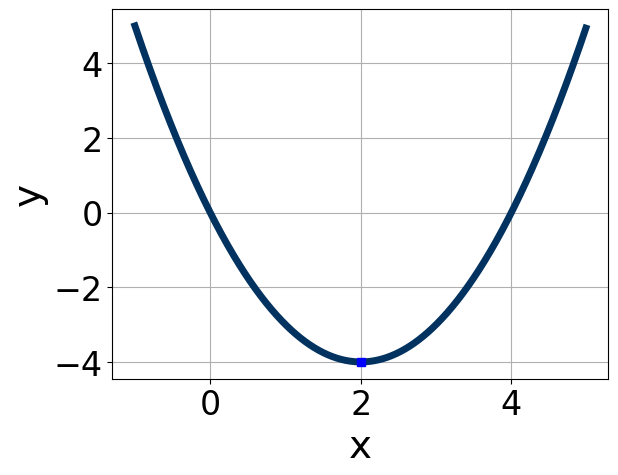
\includegraphics[width=0.5\textwidth]{../Figures/quadraticGraphToEquationB.png}
\end{center}
\begin{enumerate}[label=\Alph*.]
\item \( a \in [-2, 0], \hspace*{5mm} b \in [4, 5], \text{ and } \hspace*{5mm} c \in [-9, -5] \)
\item \( a \in [1, 5], \hspace*{5mm} b \in [4, 5], \text{ and } \hspace*{5mm} c \in [-1, 6] \)
\item \( a \in [-2, 0], \hspace*{5mm} b \in [-5, -3], \text{ and } \hspace*{5mm} c \in [-9, -5] \)
\item \( a \in [1, 5], \hspace*{5mm} b \in [-5, -3], \text{ and } \hspace*{5mm} c \in [-1, 6] \)
\item \( a \in [1, 5], \hspace*{5mm} b \in [4, 5], \text{ and } \hspace*{5mm} c \in [6, 9] \)

\end{enumerate} }
\litem{
Factor the quadratic below. Then, choose the intervals that contain the constants in the form $(ax+b)(cx+d); b \leq d.$\[ 81x^{2} -81 x + 20 \]\begin{enumerate}[label=\Alph*.]
\item \( a \in [8.8, 12.9], \hspace*{5mm} b \in [-8, -1], \hspace*{5mm} c \in [7.6, 10.7], \text{ and } \hspace*{5mm} d \in [-5, -1] \)
\item \( a \in [0.7, 2.9], \hspace*{5mm} b \in [-48, -41], \hspace*{5mm} c \in [-2.4, 1.9], \text{ and } \hspace*{5mm} d \in [-40, -32] \)
\item \( a \in [26, 30.4], \hspace*{5mm} b \in [-8, -1], \hspace*{5mm} c \in [2, 4.6], \text{ and } \hspace*{5mm} d \in [-5, -1] \)
\item \( a \in [1.4, 3.8], \hspace*{5mm} b \in [-8, -1], \hspace*{5mm} c \in [25.5, 27.8], \text{ and } \hspace*{5mm} d \in [-5, -1] \)
\item \( \text{None of the above.} \)

\end{enumerate} }
\litem{
Write the equation of the graph presented below in the form $f(x)=ax^2+bx+c$, assuming  $a=1$ or $a=-1$. Then, choose the intervals that $a, b,$ and $c$ belong to.
\begin{center}
    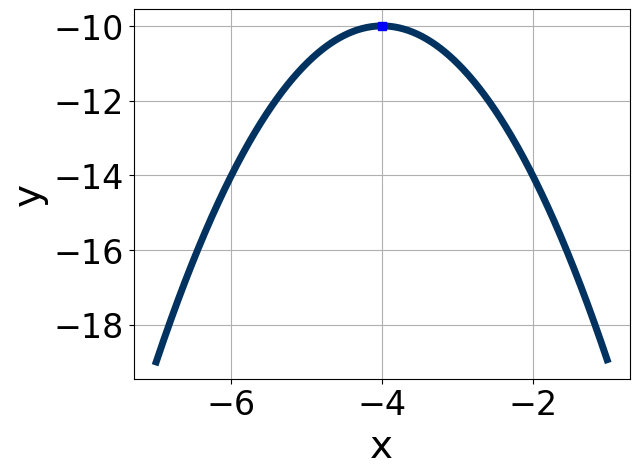
\includegraphics[width=0.5\textwidth]{../Figures/quadraticGraphToEquationCopyB.png}
\end{center}
\begin{enumerate}[label=\Alph*.]
\item \( a \in [-2, 0], \hspace*{5mm} b \in [-8, -7], \text{ and } \hspace*{5mm} c \in [-27, -23] \)
\item \( a \in [-2, 0], \hspace*{5mm} b \in [8, 11], \text{ and } \hspace*{5mm} c \in [-6, -4] \)
\item \( a \in [1, 4], \hspace*{5mm} b \in [-8, -7], \text{ and } \hspace*{5mm} c \in [6, 7] \)
\item \( a \in [1, 4], \hspace*{5mm} b \in [8, 11], \text{ and } \hspace*{5mm} c \in [6, 7] \)
\item \( a \in [-2, 0], \hspace*{5mm} b \in [8, 11], \text{ and } \hspace*{5mm} c \in [-27, -23] \)

\end{enumerate} }
\litem{
Solve the quadratic equation below. Then, choose the intervals that the solutions belong to, with $x_1 \leq x_2$ (if they exist).\[ -15x^{2} -12 x + 8 = 0 \]\begin{enumerate}[label=\Alph*.]
\item \( x_1 \in [-7.8, -4.5] \text{ and } x_2 \in [17.7, 19.6] \)
\item \( x_1 \in [-26.2, -24.5] \text{ and } x_2 \in [23.4, 24.7] \)
\item \( x_1 \in [-2.3, -0.5] \text{ and } x_2 \in [0.3, 1] \)
\item \( x_1 \in [-0.9, 0.4] \text{ and } x_2 \in [0.6, 1.4] \)
\item \( \text{There are no Real solutions.} \)

\end{enumerate} }
\litem{
Graph the equation below.\[ f(x) = -(x-4)^2 + 16 \]\begin{enumerate}[label=\Alph*.]
\begin{multicols}{2}\item 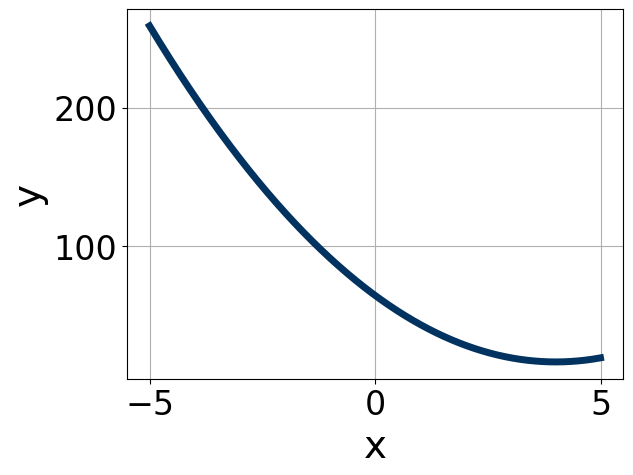
\includegraphics[width = 0.3\textwidth]{../Figures/quadraticEquationToGraphCopyAB.png}\item 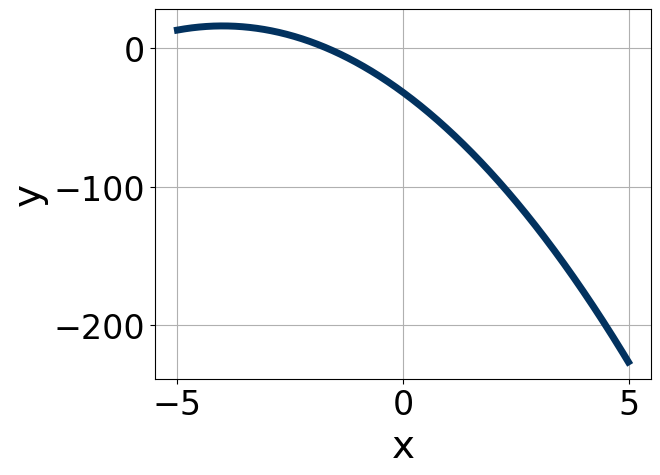
\includegraphics[width = 0.3\textwidth]{../Figures/quadraticEquationToGraphCopyBB.png}\item 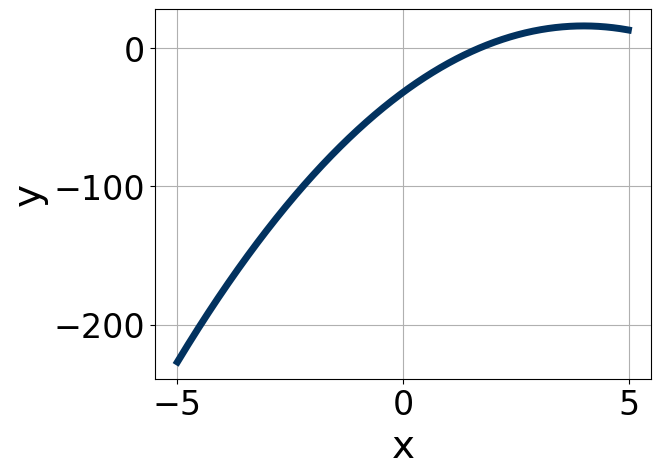
\includegraphics[width = 0.3\textwidth]{../Figures/quadraticEquationToGraphCopyCB.png}\item 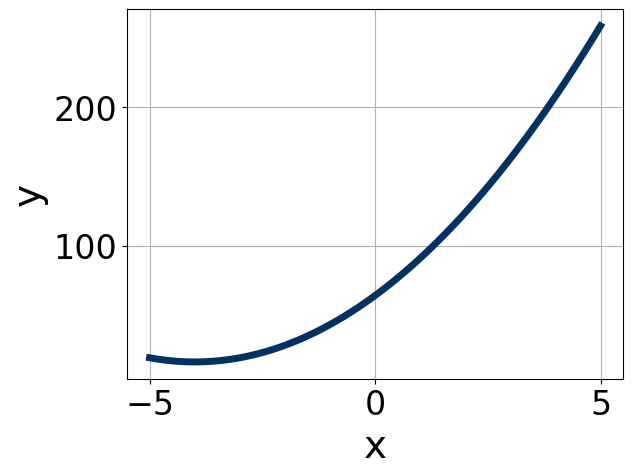
\includegraphics[width = 0.3\textwidth]{../Figures/quadraticEquationToGraphCopyDB.png}\end{multicols}\item None of the above.
\end{enumerate} }
\litem{
Solve the quadratic equation below. Then, choose the intervals that the solutions belong to, with $x_1 \leq x_2$ (if they exist).\[ -11x^{2} +11 x + 8 = 0 \]\begin{enumerate}[label=\Alph*.]
\item \( x_1 \in [-0.49, 0.51] \text{ and } x_2 \in [0.84, 1.56] \)
\item \( x_1 \in [-24.25, -20.25] \text{ and } x_2 \in [22.04, 23.11] \)
\item \( x_1 \in [-18.37, -14.37] \text{ and } x_2 \in [4.87, 5.5] \)
\item \( x_1 \in [-5.49, -0.49] \text{ and } x_2 \in [0.36, 1.22] \)
\item \( \text{There are no Real solutions.} \)

\end{enumerate} }
\litem{
Solve the quadratic equation below. Then, choose the intervals that the solutions $x_1$ and $x_2$ belong to, with $x_1 \leq x_2$.\[ 25x^{2} -60 x + 36 = 0 \]\begin{enumerate}[label=\Alph*.]
\item \( x_1 \in [0.12, 0.39] \text{ and } x_2 \in [5.23, 7.41] \)
\item \( x_1 \in [0.51, 0.71] \text{ and } x_2 \in [1.48, 2.88] \)
\item \( x_1 \in [0.38, 0.53] \text{ and } x_2 \in [2.79, 5.33] \)
\item \( x_1 \in [1.08, 1.33] \text{ and } x_2 \in [0.17, 2.27] \)
\item \( x_1 \in [29.88, 30.1] \text{ and } x_2 \in [28.99, 30.05] \)

\end{enumerate} }
\litem{
Solve the quadratic equation below. Then, choose the intervals that the solutions $x_1$ and $x_2$ belong to, with $x_1 \leq x_2$.\[ 15x^{2} -2 x -24 = 0 \]\begin{enumerate}[label=\Alph*.]
\item \( x_1 \in [-6.73, -5.44] \text{ and } x_2 \in [0.25, 0.33] \)
\item \( x_1 \in [-3.72, -3.18] \text{ and } x_2 \in [0.28, 0.61] \)
\item \( x_1 \in [-18.11, -17.49] \text{ and } x_2 \in [20, 20.03] \)
\item \( x_1 \in [-1.14, -0.44] \text{ and } x_2 \in [2.49, 2.72] \)
\item \( x_1 \in [-1.22, -0.84] \text{ and } x_2 \in [1.32, 1.48] \)

\end{enumerate} }
\litem{
Graph the equation below.\[ f(x) = (x-3)^2 + 12 \]\begin{enumerate}[label=\Alph*.]
\begin{multicols}{2}\item 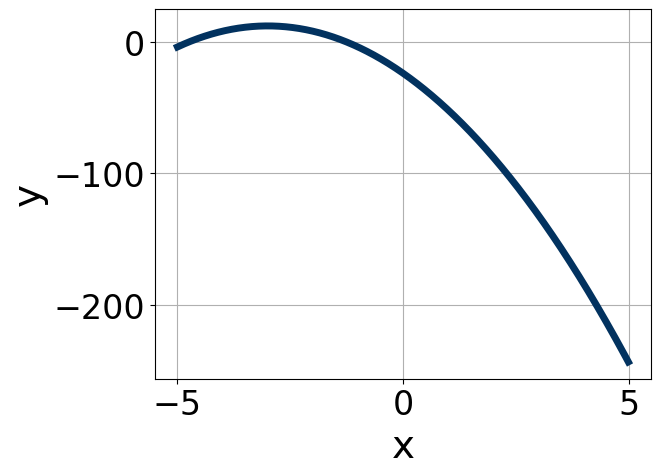
\includegraphics[width = 0.3\textwidth]{../Figures/quadraticEquationToGraphAB.png}\item 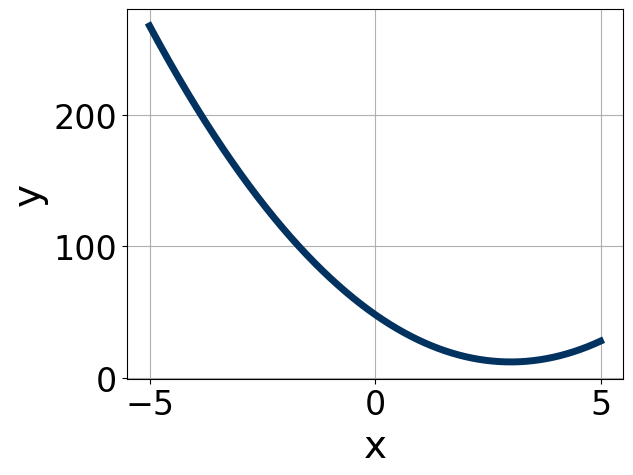
\includegraphics[width = 0.3\textwidth]{../Figures/quadraticEquationToGraphBB.png}\item 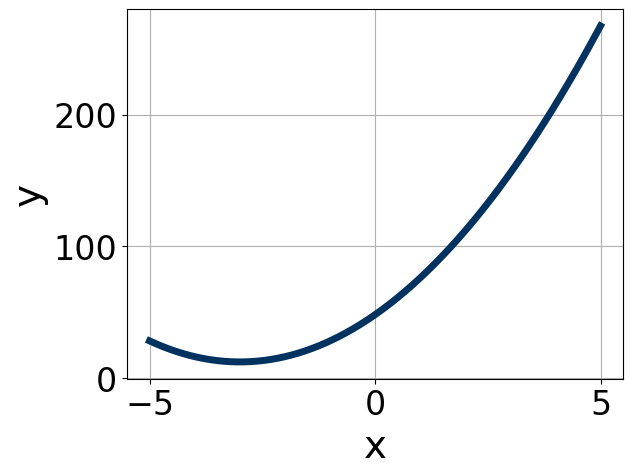
\includegraphics[width = 0.3\textwidth]{../Figures/quadraticEquationToGraphCB.png}\item 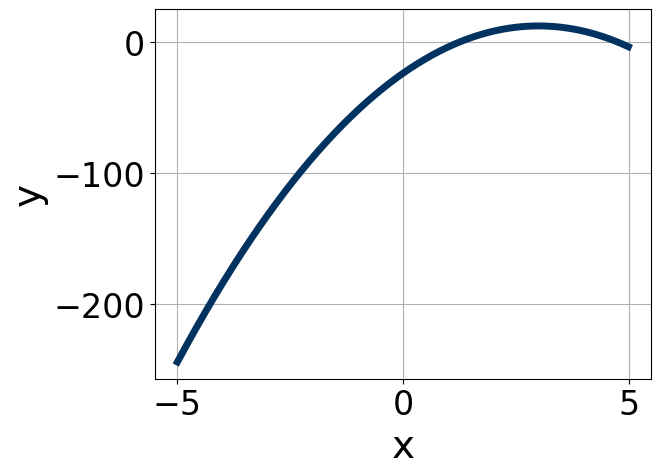
\includegraphics[width = 0.3\textwidth]{../Figures/quadraticEquationToGraphDB.png}\end{multicols}\item None of the above.
\end{enumerate} }
\end{enumerate}

\end{document}